% Vietnamese translation for OI Public Library
% Source-PDF: 图论 GRAPH THEORY/网络流题选讲 - 李宇亮.pdf
\documentclass[11pt]{article}
\usepackage{oipl-vn}
\usepackage{tikz}

\usetikzlibrary{arrows.meta,positioning}
\renewcommand{\figurename}{Hình}

\title{Tuyển giảng bài tập luồng mạng}
\author{Li Yuliang}
\date{}

\begin{document}
\maketitle

\origtitle{Selected problems on network flow}
\sourcepath{Graph Theory / Network-flow selected problems - Li Yuliang.pdf}

\section*{Lời dẫn}

Bản gốc là một bộ slide ngắn, tập trung vào cách nhận ra mô hình luồng mạng
trong các bài toán có vẻ không trực tiếp liên quan đến luồng. Phần dưới đây
viết lại thành ghi chú dạng bài giảng: với mỗi bài toán, ta nêu yêu cầu, mô
hình hóa các đỉnh và cạnh, rồi giải thích vì sao mô hình đó biểu diễn đúng
ràng buộc của đề. Các ví dụ số và sơ đồ chính trong slide được giữ lại dưới
dạng công thức, bảng hoặc hình TikZ gọn.

\section{Câu chuyện sói và cừu}

\subsection*{Đề bài}

Cho một lưới $n\times m$. Mỗi ô là sói, cừu, hoặc ô trống. Ta cần dựng hàng
rào trên biên giữa hai ô kề cạnh sao cho mọi sói bị tách khỏi mọi cừu. Hỏi số
đoạn hàng rào ít nhất cần dựng là bao nhiêu?

\subsection*{Mô hình lát cắt nhỏ nhất}

Tạo một đỉnh cho mỗi ô. Thêm nguồn $s$ và đích $t$.

\begin{itemize}
  \item Với mỗi ô chứa sói, thêm cạnh $s\to v$ có dung lượng $+\infty$.
  \item Với mỗi ô chứa cừu, thêm cạnh $v\to t$ có dung lượng $+\infty$.
  \item Với mỗi cặp ô kề cạnh, thêm một cạnh vô hướng dung lượng $1$; trong
  cài đặt luồng có thể thay bằng hai cung ngược chiều cùng dung lượng $1$,
  hoặc dùng cạnh tương đương trong mô hình lát cắt.
\end{itemize}

Khi lấy một lát cắt $s$--$t$, mọi ô sói buộc phải nằm phía nguồn, mọi ô cừu
buộc phải nằm phía đích; nếu không lát cắt sẽ phải cắt một cạnh dung lượng
$+\infty$. Những cạnh dung lượng $1$ bị cắt chính là các biên giữa hai ô mà ta
phải dựng hàng rào. Vì vậy giá trị lát cắt nhỏ nhất đúng bằng số đoạn hàng rào
ít nhất.

\section{Transform Matrix}

\subsection*{Đề bài}

Cho hai ma trận nhị phân $A$ và $B$ kích thước $n\times m$. Ta được thực hiện
một số phép đổi chỗ hai phần tử ở hai ô kề cạnh trong $A$, sao cho cuối cùng
$A$ trở thành $B$. Mỗi ô $(i,j)$ được tham gia vào không quá
$\operatorname{count}(i,j)$ phép đổi chỗ. Hỏi tổng số phép đổi chỗ nhỏ nhất.

Trước hết, nếu số lượng ô bằng $1$ trong hai ma trận khác nhau thì bài toán vô
nghiệm. Phần dưới giả sử hai số lượng này bằng nhau.

\subsection*{Không xét giới hạn số lần dùng ô}

Một phép đổi chỗ kề cạnh có thể nhìn như việc di chuyển một đơn vị ``$1$'' qua
một cạnh của lưới, với chi phí $1$. Khi đã biết các vị trí ban đầu và cuối
cùng của các số $1$, bài toán trở thành ghép từng số $1$ ban đầu với một vị
trí đích sao cho tổng khoảng cách Manhattan nhỏ nhất. Mô hình luồng chi phí
nhỏ nhất như sau.

\begin{itemize}
  \item Với mỗi ô $v$ có $A_v=1$, thêm cạnh $s\to v$ dung lượng $1$, chi phí
  $0$.
  \item Với mỗi ô $v$ có $B_v=1$, thêm cạnh $v\to t$ dung lượng $1$, chi phí
  $0$.
  \item Với mỗi cặp ô kề cạnh $u,v$, thêm hai cung $u\to v$ và $v\to u$, dung
  lượng $+\infty$, chi phí $1$.
\end{itemize}

Gửi toàn bộ số đơn vị $1$ từ nguồn đến đích. Mỗi đường đi của một đơn vị luồng
tương ứng với lộ trình của một số $1$, và chi phí đường đi là số phép đổi chỗ
cần dùng.

\subsection*{Thêm giới hạn \texorpdfstring{\(\operatorname{count}\)}{count}}

Giới hạn số lần một ô được thao tác là một ràng buộc qua đỉnh. Ta tách mỗi ô
$v$ thành $v_{\mathrm{in}}$ và $v_{\mathrm{out}}$, nối
$v_{\mathrm{in}}\to v_{\mathrm{out}}$ bằng cạnh chi phí $0$ và dung lượng
phụ thuộc vào trạng thái của ô.

\[
  b_v=
  \begin{cases}
    \left\lfloor \operatorname{count}(v)/2\right\rfloor,
      & A_v=B_v,\\[0.4em]
    \left\lfloor(\operatorname{count}(v)+1)/2\right\rfloor,
      & A_v\ne B_v.
  \end{cases}
\]

Lý do là nếu $A_v=B_v$, số lần đi vào và đi ra khỏi ô phải cân bằng nên các
thao tác tại ô xuất hiện theo cặp. Nếu $A_v=1,B_v=0$, ô này có một lần đi ra
nhiều hơn đi vào; nếu $A_v=0,B_v=1$, ô này có một lần đi vào nhiều hơn đi ra.
Hai trường hợp sau đều cho phép thêm một lần lẻ, nên dung lượng là
$\lfloor(\operatorname{count}(v)+1)/2\rfloor$.

Các cạnh kề cạnh của lưới được nối từ $u_{\mathrm{out}}$ sang
$v_{\mathrm{in}}$ và ngược lại, dung lượng $+\infty$, chi phí $1$. Cạnh nguồn
và cạnh đích nối vào các nửa đỉnh tương ứng. Sau khi tách đỉnh, luồng chi phí
nhỏ nhất tự động chọn các đường đi vừa rẻ nhất vừa không vượt quá số lần mỗi ô
được dùng.

\section{Road}

\subsection*{Đề bài}

Cho dãy độ cao $h_1,h_2,\ldots,h_n$. Ta được thay đổi các phần tử, với chi phí
tổng cộng
\[
  \sum_i |\Delta h_i|.
\]
Cần làm cho mọi hiệu hai phần tử kề nhau có trị tuyệt đối không vượt quá $d$,
tức
\[
  |h_i-h_{i+1}|\le d \qquad (1\le i<n),
\]
và cần cực tiểu hóa chi phí sửa đổi.

\subsection*{Chuyển sang phân phối lại hiệu}

Đặt
\[
  a_i=h_i-h_{i+1}\qquad (1\le i<n).
\]
Khi tăng $h_i$ thêm $1$ với $1<i<n$, ta làm $a_{i-1}$ giảm $1$ và $a_i$ tăng
$1$. Nói cách khác, một đơn vị được chuyển giữa hai hiệu kề nhau, và chi phí
là $1$. Giảm $h_i$ thêm $1$ cho chuyển động ngược lại. Vì vậy mục tiêu là
phân phối lại các đơn vị trên dãy $a$ sao cho mọi $a_i$ nằm trong đoạn
$[-d,d]$.

Tạo một đỉnh cho mỗi $a_i$. Giữa hai đỉnh kề nhau, thêm hai cung ngược chiều
dung lượng $+\infty$, chi phí $1$. Một đơn vị luồng đi qua cung này biểu diễn
một lần sửa một phần tử ở giữa.

\subsection*{Ràng buộc trên từng hiệu}

Với mỗi $a_i$, lượng ròng cần lấy đi hoặc thêm vào được biểu diễn bằng các
cạnh nối với nguồn và đích.

\begin{itemize}
  \item Nếu $a_i>d$, ta phải lấy đi ít nhất $a_i-d$ đơn vị, và có thể lấy đi
  nhiều nhất $a_i+d$ đơn vị trước khi vượt quá biên dưới $-d$. Thêm cạnh
  $s\to i$ có cận dưới $a_i-d$, cận trên $a_i+d$, chi phí $0$.
  \item Nếu $a_i<-d$, ta phải bù vào ít nhất $-d-a_i$ đơn vị, và có thể bù
  nhiều nhất $d-a_i$ đơn vị. Thêm cạnh $i\to t$ có cận dưới $-d-a_i$, cận trên
  $d-a_i$, chi phí $0$.
  \item Nếu $-d\le a_i\le d$, cả hai hướng đều có thể xảy ra: thêm cạnh
  $s\to i$ cận trên $a_i+d$ và cạnh $i\to t$ cận trên $d-a_i$, đều có cận dưới
  $0$ và chi phí $0$.
\end{itemize}

Hai đầu dãy là trường hợp đặc biệt. Sửa $h_1$ chỉ ảnh hưởng đến $a_1$, còn sửa
$h_n$ chỉ ảnh hưởng đến $a_{n-1}$. Vì thế đơn vị có thể xuất hiện hoặc biến
mất ở hai đầu với chi phí $1$: thêm các cạnh $s\to 1$, $1\to t$,
$s\to n-1$, $(n-1)\to t$ dung lượng $+\infty$, chi phí $1$.

Mạng thu được là một bài toán \term{luồng khả thi chi phí nhỏ nhất} có cận
dưới. Chi phí của luồng chính là tổng số lần tăng hoặc giảm các phần tử của
dãy $h$.

\section{Xây dựng Utopia}

\subsection*{Đề bài}

Cho một đồ thị gồm các đỉnh đặc biệt và các đỉnh thường; mỗi cạnh có ít nhất
một đầu mút là đỉnh đặc biệt. Mỗi đỉnh có một giá trị nguyên $L$ trong đoạn
$1$ đến $20$. Giá trị của đỉnh đặc biệt có thể sửa, với chi phí
$c|L'_i-L_i|$. Mỗi cạnh $(i,j)$ đóng góp chi phí $e|L'_i-L'_j|$, trong đó
đỉnh thường giữ nguyên giá trị ban đầu. Cần cực tiểu hóa tổng chi phí.

\subsection*{Tách phần chỉ phụ thuộc vào một đỉnh}

Trước hết bỏ qua các cạnh nối giữa hai đỉnh đặc biệt. Với mỗi đỉnh đặc biệt
$i$ và mỗi giá trị $k\in\{1,2,\ldots,20\}$, đặt
\[
  \operatorname{cost}_{i,k}
  = c|k-L_i|+
  e\sum_{\substack{j\text{ là đỉnh thường}\\ (i,j)\text{ là cạnh}}}
    |k-L_j|.
\]
Nếu không có cạnh giữa hai đỉnh đặc biệt, chỉ cần chọn độc lập giá trị $k$ có
\(\operatorname{cost}_{i,k}\) nhỏ nhất cho từng đỉnh đặc biệt.

\subsection*{Cạnh giữa các đỉnh đặc biệt}

Khi có cạnh giữa hai đỉnh đặc biệt, bài toán trở thành
\[
  \min \left\{
    \sum_i \operatorname{cost}_{i,x_i}
    + e\sum_{(i,j)} |x_i-x_j|
  \right\},
  \qquad x_i\in\{1,2,\ldots,20\},
\]
trong đó tổng thứ hai chỉ tính trên các cạnh nối hai đỉnh đặc biệt.

Slide minh họa trường hợp đơn giản có ba đỉnh đặc biệt tạo thành đường
\((1,2),(2,3)\) và bốn mức giá trị. Nếu chọn
\[
  L'_1=4,\qquad L'_2=2,\qquad L'_3=3,
\]
thì phần chi phí cạnh đặc biệt--đặc biệt là
\[
  e\bigl(|4-2|+|2-3|\bigr)=e(2+1),
\]
còn phần chi phí một đỉnh là
\[
  c\sum_i \operatorname{cost}_{i,L'_i}.
\]
Trong cách nhìn theo lớp, hai cột của đỉnh \(1\) và \(2\) khác nhau ở hai
lớp, còn hai cột của đỉnh \(2\) và \(3\) khác nhau ở một lớp; chính các lớp
khác nhau này tạo ra chi phí \(e|x_i-x_j|\).

Đây là một mô hình gán nhãn có thứ tự và có thể dựng bằng lát cắt nhỏ nhất
theo lớp. Với mỗi đỉnh đặc biệt $i$, tạo các biến nhị phân
\[
  y_{i,\ell}=[x_i>\ell]\qquad (1\le \ell<20).
\]
Thêm các cạnh dung lượng $+\infty$ để ép chuỗi đơn điệu
\[
  y_{i,\ell+1}=1\Rightarrow y_{i,\ell}=1.
\]
Như vậy mọi lát cắt hữu hạn tương ứng đúng với một giá trị $x_i$.

Phần chi phí một đỉnh được đưa vào các cạnh nối nguồn/đích theo sai phân
\[
  \Delta_{i,\ell}=
  \operatorname{cost}_{i,\ell+1}-\operatorname{cost}_{i,\ell}.
\]
Nếu \(\Delta_{i,\ell}>0\), thêm cạnh từ biến \(y_{i,\ell}\) đến đích có dung
lượng \(\Delta_{i,\ell}\); nếu \(\Delta_{i,\ell}<0\), thêm cạnh từ nguồn đến
\(y_{i,\ell}\) có dung lượng \(-\Delta_{i,\ell}\). Hằng số
\(\operatorname{cost}_{i,1}\) không ảnh hưởng đến vị trí lát cắt và chỉ cần
cộng lại vào đáp án.

Với mỗi cạnh đặc biệt--đặc biệt $(i,j)$ và mỗi mức \(\ell\), thêm một cạnh vô
hướng dung lượng \(e\) giữa \(y_{i,\ell}\) và \(y_{j,\ell}\). Số mức mà hai
dãy nhị phân khác nhau đúng bằng \(|x_i-x_j|\), nên tổng dung lượng bị cắt
trên các cạnh này là \(e|x_i-x_j|\). Do đó lát cắt nhỏ nhất cho ta phương án
sửa các giá trị \(L\) tối ưu.

\section{Giải đấu vòng tròn}

\subsection*{Đề bài}

Trong một giải đấu vòng tròn một lượt, mỗi cặp đấu có đúng một người thắng và
không có hòa. Một số kết quả đã biết trước. Hỏi những người nào còn có thể
trở thành nhà vô địch, tức có số trận thắng không nhỏ hơn mọi người khác sau
khi gán kết quả cho các trận chưa đấu?

\subsection*{Mô hình khả thi bằng luồng cực đại}

Ta xét riêng một ứng viên $p$. Ép $p$ thắng tất cả các trận còn lại của mình;
khi đó số trận thắng cuối cùng của $p$ đã xác định, gọi là \(W_p\). Các trận
còn lại chỉ là các trận giữa những người khác.

Với một ngưỡng \(k\le W_p\), kiểm tra xem có thể gán người thắng cho các trận
còn lại sao cho mọi người khác thắng không quá \(k\) trận hay không. Dựng mạng
hai phía:

\begin{itemize}
  \item Mỗi trận chưa biết giữa hai người khác $u,v$ là một đỉnh trận đấu.
  \item Mỗi người chơi khác $p$ là một đỉnh người chơi.
  \item Thêm cạnh $s\to g$ dung lượng $1$ cho mỗi đỉnh trận đấu $g$.
  \item Từ $g$ nối đến hai người chơi tham gia trận đó, mỗi cạnh dung lượng
  $1$.
  \item Nếu người chơi $i$ hiện đã có $w_i$ trận thắng, thêm cạnh
  $i\to t$ dung lượng \(k-w_i\). Nếu \(k<w_i\), ngưỡng này bất khả thi ngay.
\end{itemize}

Nếu luồng cực đại bão hòa mọi cạnh đi ra từ nguồn, mỗi đơn vị luồng chọn đúng
một người thắng cho một trận, và dung lượng cạnh \(i\to t\) bảo đảm người đó
không vượt quá \(k\) trận thắng. Có thể nhị phân \(k\), hoặc trong bài toán
chỉ cần biết ứng viên \(p\) có thể vô địch thì thử trực tiếp \(k=W_p\). Nếu đề
yêu cầu vô địch tuyệt đối không đồng hạng, thay \(k\) bằng \(W_p-1\).

\section{Tuyển mộ tình nguyện viên}

\subsection*{Đề bài}

Có $N$ ngày. Ngày thứ $i$ cần ít nhất \(a_i\) tình nguyện viên. Có \(M\) loại
tình nguyện viên; loại thứ \(j\) có số lượng không hạn chế, làm việc liên tục
từ ngày \(s_j\) đến ngày \(t_j\), và mỗi người thuộc loại này có chi phí
\(c_j\). Cần đạt đủ nhu cầu mỗi ngày với tổng chi phí nhỏ nhất.

Ví dụ trong slide:
\[
\begin{array}{l}
N=3,\quad M=3,\\
a=(2,3,4),\\
\text{khoảng }[1,2]\ \text{có chi phí }2,\qquad
\text{khoảng }[2,3]\ \text{có chi phí }5,\qquad
\text{khoảng }[3,3]\ \text{có chi phí }2.
\end{array}
\]
Nếu gọi ba biến chọn loại tình nguyện viên là \(X_1,X_2,X_3\), các ràng buộc
ban đầu là
\[
  X_1\ge 2,\qquad X_1+X_2\ge 3,\qquad X_2+X_3\ge 4.
\]

\subsection*{Từ bất đẳng thức sang cân bằng luồng}

Gọi \(X_j\) là số người chọn từ loại \(j\). Ràng buộc ngày \(i\) là
\[
  \sum_{j:s_j\le i\le t_j} X_j \ge a_i.
\]
Đưa biến dư \(Y_i\ge 0\) vào, ta có
\[
  \sum_{j:s_j\le i\le t_j} X_j - Y_i = a_i.
\]
Lấy hiệu giữa hai phương trình liên tiếp. Khi đó mỗi biến \(X_j\) chỉ còn
xuất hiện đúng hai lần: một lần với dấu dương tại ngày \(s_j\), và một lần
với dấu âm ngay sau ngày \(t_j\). Mỗi biến dư \(Y_i\) cũng xuất hiện hai lần,
một âm và một dương. Đây chính là dạng cân bằng luồng.

Với ví dụ trên, sau khi thêm biến dư rồi lấy hiệu, slide thu được hệ:
\[
\begin{aligned}
X_1-Y_1-2&=0,\\
Y_1+X_2-Y_2-1&=0,\\
-X_1+Y_2+X_3-Y_3-1&=0,\\
-X_2-X_3+Y_3+4&=0.
\end{aligned}
\]
Mỗi biến \(X\) hoặc \(Y\) xuất hiện đúng hai lần, một lần dấu dương và một
lần dấu âm, nên có thể xem biến đó là một cạnh chảy từ phương trình này sang
phương trình kia.

Tạo các đỉnh \(1,2,\ldots,N+1\), tương ứng với các phương trình sau khi lấy
hiệu. Với mỗi loại tình nguyện viên \(j\), thêm cạnh
\[
  s_j\to t_j+1
\]
dung lượng \(+\infty\), chi phí \(c_j\). Với mỗi biến dư \(Y_i\), thêm cạnh
\[
  i+1\to i
\]
dung lượng \(+\infty\), chi phí \(0\). Các hằng số ở vế phải tạo thành nhu cầu
cân bằng tại từng đỉnh:
\[
  b_1=a_1,\qquad b_i=a_i-a_{i-1}\ (2\le i\le N),\qquad b_{N+1}=-a_N.
\]
Đỉnh có \(b_i>0\) cần phát ra \(b_i\) đơn vị ròng, đỉnh có \(b_i<0\) cần nhận
\(-b_i\) đơn vị ròng. Thêm siêu nguồn và siêu đích để thỏa các cân bằng này,
rồi giải luồng khả thi chi phí nhỏ nhất. Chi phí của các cạnh loại tình
nguyện viên đúng bằng tổng chi phí tuyển người.

\section{Đoạn thẳng phủ không quá \texorpdfstring{\(k\)}{k} lần}

\subsection*{Đề bài}

Cho \(N\) khoảng mở trên trục số. Chọn một số khoảng sao cho không có điểm nào
bị phủ bởi quá \(k\) khoảng đã chọn. Hãy cực đại hóa tổng độ dài các khoảng
được chọn.

\subsection*{Mô hình luồng chi phí lớn nhất}

Rời rạc hóa tất cả đầu mút và sắp chúng theo thứ tự tăng dần. Tạo một đỉnh
cho mỗi tọa độ rời rạc, thêm nguồn \(s\) nối đến tọa độ đầu tiên và tọa độ
cuối cùng nối đến đích \(t\), đều có dung lượng \(k\), chi phí \(0\).

Giữa hai tọa độ liên tiếp, thêm cạnh đi từ trái sang phải, dung lượng \(k\),
chi phí \(0\). Với mỗi khoảng \((l,r)\), thêm cạnh từ đỉnh của \(l\) đến đỉnh
của \(r\), dung lượng \(1\), chi phí bằng độ dài \(r-l\). Sau đó tìm luồng cực
đại chi phí lớn nhất gồm \(k\) đơn vị từ trái sang phải.

\begin{figure}[ht]
\centering
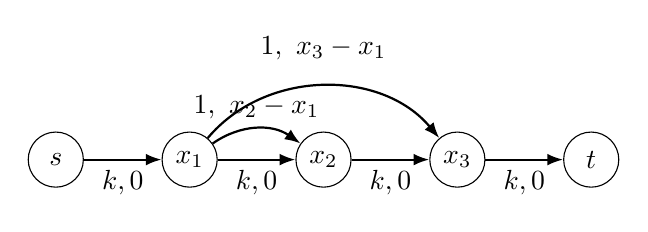
\begin{tikzpicture}[
  x=1cm,y=1cm,
  v/.style={circle,draw,minimum size=7mm,inner sep=0pt},
  arc/.style={-{Latex[length=2mm]},thick}
]
  \node[v] (s) at (0,0) {$s$};
  \node[v] (x1) at (1.7,0) {$x_1$};
  \node[v] (x2) at (3.4,0) {$x_2$};
  \node[v] (x3) at (5.1,0) {$x_3$};
  \node[v] (t) at (6.8,0) {$t$};
  \draw[arc] (s) -- node[below] {\(k,0\)} (x1);
  \draw[arc] (x1) -- node[below] {\(k,0\)} (x2);
  \draw[arc] (x2) -- node[below] {\(k,0\)} (x3);
  \draw[arc] (x3) -- node[below] {\(k,0\)} (t);
  \draw[arc,bend left=35] (x1) to node[above] {\(1,\ x_2-x_1\)} (x2);
  \draw[arc,bend left=50] (x1) to node[above=2mm] {\(1,\ x_3-x_1\)} (x3);
\end{tikzpicture}
\caption{Mạng sau khi rời rạc hóa: cạnh chuỗi có dung lượng \(k\), cạnh khoảng có dung lượng \(1\) và chi phí bằng độ dài khoảng.}
\end{figure}

Mỗi đơn vị luồng biểu diễn một lớp phủ. Cạnh khoảng có dung lượng \(1\), nên
mỗi khoảng được chọn nhiều nhất một lần; dung lượng \(k\) trên các cạnh nối
hai tọa độ liên tiếp bảo đảm tại mọi đoạn nhỏ giữa hai đầu mút, nhiều nhất
\(k\) khoảng được chọn phủ qua đó. Chi phí tối đa chính là tổng độ dài lớn
nhất cần tìm. Nếu chỉ có thuật toán luồng chi phí nhỏ nhất, đổi dấu chi phí
của các cạnh khoảng.

\section*{Kết luận}

Các ví dụ trên đều có chung một nhịp: xác định đại lượng nào cần được bảo toàn
hoặc phân phối, biến lựa chọn cục bộ thành cạnh có dung lượng, và để lát cắt
hoặc luồng chi phí xử lý phần tối ưu. Những bài tưởng như là sửa dãy, đổi ma
trận, gán kết quả thi đấu hay chọn khoảng đều có thể đưa về cùng vài mẫu mô
hình: lát cắt nhỏ nhất, luồng cực đại kiểm tra khả thi, và luồng chi phí nhỏ
nhất hoặc lớn nhất.

\end{document}
